\documentclass[letterpaper,twocolumn,10pt]{article}
\usepackage{usenix,epsfig,endnotes}
\usepackage{enumitem}
\usepackage{url}
\usepackage{graphicx}
\usepackage{color}
\usepackage[usenames,dvipsnames]{xcolor}
\usepackage{booktabs}
\usepackage{caption}
\usepackage{subcaption}
\usepackage{color,soul}
\usepackage{marginnote}
\usepackage{framed}
\usepackage{balance}
\usepackage{amsmath}
\usepackage{algorithm} %ctan.org\pkg\algorithms
\usepackage{algpseudocode}

\definecolor{myyellow}{rgb}{1.0, 0.98, 0.77}
\sethlcolor{myyellow}

\setlength{\marginparwidth}{0.5in}

\begin{document}

%don't want date printed
\date{}

%some useful commands
\newcommand{\name}{gHyvi}
\newcommand{\gvirt}{gVirt}
\newcommand{\RNum}[1]{\uppercase\expandafter{\romannumeral #1\relax}}
\newcommand{\vm}{{Virtual Machine~(VM)}\renewcommand{\vm}{VM}}
\newcommand{\gpu}{{Graphic Process Unit~(GPU)}\renewcommand{\gpu}{GPU}}
\newcommand{\gpgpu}{{General-purpose computing on graphics processing units~(GPGPU)}\renewcommand{\gpu}{GPGPU}}
\newcommand{\ppgtt}{page table}
\newcommand{\benchmark}{GMedia}


%make title bold and 14 pt font (Latex default is non-bold, 16 pt)
\title{\Large \bf A modified ingress controller for Kubernetes}

%for single author (just remove % characters)
\author{
{\rm Jianxin Zhang\textsuperscript{1}}\\
\{zjx556\}@sjtu.edu.cn\\
\textsuperscript{1}Shanghai Jiao Tong University
% copy the following lines to add more authors
% \and
% {\rm Name}\\
%Name Institution
} % end author


\maketitle

% Use the following at camera-ready time to suppress page numbers.
% Comment it out when you first submit the paper for review.
%\thispagestyle{empty}

\subsection*{Abstract}
\hspace{0pt}
Recently web applications have grown explosively with the widespread of internet and networking devices. Many applications rely on container-base cluster to provide stability and high performance. For a specific application, given thought to diverse resource consumption (such as CPU, memory, etc.) and frequency of different kinds of requests, it is difficult to balance load of servers. So problems like performance degradation will be caused ineluctably if too many requests are sent to over-load servers. In this paper, a dynamic load balance algorithm which takes request consumption and server load into account is proposed to reduce the performance problem. Experimental results are given to validate the performance of proposed algorithm.


\section{Introduction}
\label{sec:introduction}

The rapid growth of internet introduces a new economy pattern named internet economy, under which almost all activities can be supported by web services through PCs or mobile devices. Aiming to achieve high resource utilization and better lifecycle management, web applications tend to be deployed into cluster based on a lightweight virtualization called container just like other traditional applications do. Unlike traditional applications which only execute job assigned in advance, web services have to listen on users'  requests and responses as soon as possible. Workload of web services are changing unpredictably because they offer varied businesses, each business consists of operations that may consume CPU, allocate memory or access disk, and it is impossible to know which business will be executed in any time. The unpredictable workload introduces a hug challenge on load-balancing. Unfortunately, the container-based solutions like Kubernetes fail to cope with this challenge, their fair load-balancing algorithm performs well only when workload are the same, which is contrary to workload of web services, as a result, web services fail to gain high resource utilization, it loses stability and performance conversely.

To address the load balance problem, this paper introduce a dynamic load-balancing solution based on Kubernetes, a popular container cluster management system. The new solution mainly covers two issues: Load collection and load-balancing algorithm.

The load collection part tries to collect information for load balancer to adjust its requests dispatching decision.For this part, we implement a load monitor to evaluate resource consumption of request types and collect load of backend containers. Through collecting and analyzing logs of web services, the monitor generates resource description for different request types, which represents their consumption of different resources. Through listening on status changes of container, monitor generates load description for usage of CPU, memory and network.

For the algorithm part, we introduce request and container models based on description generated by monitor. The generation of models considers not only the load description, but also other details such as the locality, deployment configuration of container and so on. Request dispatching is done through matching request models to container models.

In summary, this paper makes the following contributions:

\begin{itemize}

\item A load monitor for learning resource consumption of requests and listening load changes of containers.

\item A dynamic load-balancing algorithm which combines resource consumption of request and real-time load of container to dispatch request and finally achieve stability, high performance and high resource utilization for web services.

\item An evaluation to show the performance of dynamic load-balancing solution.
 % \item A \gpu{}-enabled benchmark for media transcoding performance (GMedia), by invoking functions from Intel MSDK to evaluate and report the  performance on Intel's \gpu{} platforms.


\end{itemize}
The rest of the paper is organized as follows: Section~\ref{sec:background} describe background information about performance of web services in container-base cluster. Section~\ref{sec:Design} presents the design and implementation of dynamic load-balancing solution. Then section~\ref{sec:evaluation} evaluate the solution. Section~\ref{sec:related_work} shows the related work, and finally section~\ref{sec:conclusion} discuss on the future work.

\section{Background}
\label{sec:background}

Performance of web services is sensitive to system metrics of their backend servers, in container-based cluster, that is backend containers. For convenience, we called the backend containers as endpoints in this paper. This section first points out factors that affect performance of web services in container-based cluster, and then introduces the current design of load-balancing solution, that is ingress controller in Kubernetes and finally state defects of ingress controller.

\subsection{Influencing factors}
\label{subsec:Influencing_factors}

Factors that affect the performance include CPU usage, memory usage, network usage, services dependency and locality.
As known to us, servers with high usage in CPU, memory or network will perform badly. Things are same when it comes to container-based cluster, for an endpoint, it causes delay on requests processing when it is high-loaded in CPU and network. More and more, if the endpoints are in high-loaded state for memory, they face the risk that they may be restarted due to OOM(out of memory) problem. Thus, if we demand high performance for web application, we'd better even load of each endpoint and reduce overhead endpoints as many as possible.
services dependency means that services do not provides functions themselves, they rely on applications of other services to finish their jobs. For example, we have endpoint1, endpoint2,endpoint3 for serviceA, and endpoint4,enpoint5 for serviceB, and serviceA relies on serviceB to process its requests, particularly, endpoint1 and endpoint2 rely on endpoint5, endpoint3 relies on endpoint5. Obviously, the performance of endpoint4 and endpoint5 will directly influence the performance of endpoint1, endpoint2 and endpoint3. Furthermore, the competition between endpoint1 and endpoint2 for accessing endpoint5 will have a negatice impact on performance of serviceA. This paper select database dependency as an example of services dependency. That is endpoints of a web service rely on endpoints of database to process requests, which is also a common case for web services. Traditionally, developers tend to reduce pressure of database by dividing it into several databases and synchronize data between them. Therefore, it is common for an endpoint to access a database that is not only the same as some endpoints, but also different from others. Under this circumstance, performance of web applications can be improved through reducing race between endpoints that share the same database or reducing the overhead endpoints of databases.
Locality means that the placement of endpoints may affect their performance. Though containers are claimed to isolate resource from each other, papers~{\cite{Zhao2018Locality}} still show that when two or more endpoints are placed in the same node, the delay appears. More and more, although under circumstance that an endpoint monopolizes a node, it still remains possibility for delay when the node is in high-load status because of some system processes. So the locality should also be considered for a better load-balancing performance.

\subsection{Ingress controller}
\label{subsec:ingress_controller}

\begin{figure}[htbp]
  \centering
  
\includegraphics[width=0.45\textwidth]{images/ingress_controller.png}\\
  \caption{Workflow of ingress controller}
  \label{fig:ingress_controller}
\end{figure}
\hspace{0pt}

Figure~{\ref{fig:ingress_controller}} shows the workflow of kubernetes load-balancing component -- ingress controller: To balance network workload, ingress controller focuses on two part, one is to keep track of the IP and number change of endpoints so that it can update traffic rules in time to guarantee accuracy. The other part is watching ingress to update load-balancing strategy. Ingress is a resource describing inbound rules for connections to reach endpoints. With correct status of endpoints and a configured ingress, ingress controller sets up appropriate traffic rules for its built-in loadbalancer(nginx). Finally, the loadbalancer dispatches requests to suitable endpoints according to configured rules, balancing load across endpoints.



\subsection{Shortcomings of ingress controller}
\label{subsec:Shortcoming}
Rather than balancing load, ingress controller concentrates more on linking ingress to nginx features like session affinity to let users to custom their load-balancing algorithm smoothly in kubernetes. However, its configurable algorithms are simply based on static algorithms like round\_robin, which do not consider influencing factors mentioned above. To summary, the igress controller has two shortcomings when it is put into pratice, that is hysteresis and one-sidedness. The round\_robin strategy assumes that all requests have the same resource consumption and aims to balance load after a long period of time, so problems come when requests change in a rather short time. For example, when there is a peak of requests, and new endpoints is needed to participate in providing service. A appropriate way to balance load now is to dispatch more workload to new idle endpoints and reduce workload for high-loaded old endpoints, but the round\_robin algorithm still dispatches requests indistinguishably, taking the riks that the old high-loaded endpoints may be unable to work normally, even restarted due to OOM although it will finally balance load relatively. The one-sideness means that the round\_robin algorithm only considers to even workload accross endpoints, without taking influencing factors mentioned above, thus failes to balance load accurately. To address these shortcomings of ingress controller, this paper presents an alternative basic algorithm to ingress controller, that is a dynamic load algorithm that takes these factors and request information into consideration.

\section{Design and implementation}
\label{sec:Design}

To overcome the shortcoming of ingress controller, this paper proposes a dynamic load-balancing solution. The solution consists of two part, one part is load monitor, the other part is dynamic load-balancing algorithm.

\subsection{Workflow}
\label{subsec:workflow}
\begin{figure}[htbp]
  \centering
  
\includegraphics[width=0.45\textwidth]{images/dynamic_solution.png}\\
  \caption{Workflow of dynamic solution}
  \label{fig:dynamic_solution}
\end{figure}
Figure~{\ref{fig:dynamic_solution}} illustrates the workflow of the dynamic load-balancing solution:
\begin{enumerate}[label=(\arabic*)]
  \item Load monitor gather necessary data for dynamic load balancing and offer data to loadbalancer.
  \item Loadbalancer makes a further evaluation for data received from loadmonitor and dispatches incoming requests based on dynamic load-balancing algorithm.
  \end{enumerate}

\subsection{Load monitor}
\label{subsec:load_monitor}

\begin{figure}[htbp]
  \centering
  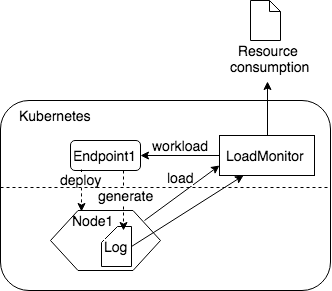
\includegraphics[width=0.45\textwidth]{images/request_learning.png}\\
  \caption{request-learing phase}
  \label{fig:request_learning}
\end{figure}

Load monitor collects, analyzes and outputs information needed by dynamic load-balancing algorithm. Load monitor processes two kinds of information: request logs and endpoint loads.
Request logs are used for evaluating resource consumption of request. Before running in kubernetes, each web service goes through the request-learning phase shown by figure~{\ref{fig:request_learning}}: First, a single endpoint is deployed, then load monitor generates workload by keep on sending requests in a fixed speed to the endpoint, the speed increases with time until it reach the processing limit of endpoint. At the same time, load monitor combines service logs, workload and endpoint load to evaluate resource description for each type of request.
We define $RD_i$ as resource description of  a $i_{st}$ type request.$C_i$ ,$M_i$ and $N_i$ stand for CPU, memory, network consumption to process a $i_{st}$ type request. $S_{i}^{t}$ stands for speed of sending $i_{st}$ type request in timestamp t. $c_{i}^{t}$, $m_{i}^{t}$, $n_{i}^{t}$ are CPU, memory, network load of endpoint in timestamp t during $i_{st}$request-learning phase. The computation of resource description is as follow:

$$ C_i = \frac{\sum_{j=1}^{k}\frac{c_{i}^{t}}{s_{i}^{t}}}{k}, M_i = \frac{\sum_{j=1}^{k}\frac{m_{i}^{t}}{s_{i}^{t}}}{k}, N_i = \frac{\sum_{j=1}^{k}\frac{n_{i}^{t}}{s_{i}^{t}}}{k}$$

$$RD_i = \left \{ C_i, M_i, N_i \right \}$$


Then load monitor enters load-collecting phase shown in figure~{\ref{fig:load_collecting}} to generate load description for endpoints.To increase load-balancing performance, load description of endpoints has to cover all influencing factors. For the resource usage part, Load monitor collects system loads from kubelet, a component that is not only responsible for managing lifecycle of pods, but also takes charge of collecting cluster load. For sharing problem and locality, load monitor obtains endpoint information from apiserver. Endpoint information includes configuration that which endpoints share the same database, which endpoints are deployed in the same node and so on. Table~{\ref{table:load_description}} is an example of load description given by load monitor.
\begin{figure}[htbp]
  \centering
  
\includegraphics[width=0.45\textwidth]{images/endpoint_load.png}\\
  \caption{load-collecting phase}
  \label{fig:load_collecting}
\end{figure}

\hspace{0pt}
\begin{table}[htbp]
 \begin{center}
  \begin{tabular}{c|c|c|c}
   \hline
   Type           & Pod    & Pod   & Node  \\  \hline
   Name           & App1   & Db1   & Node1 \\ \hline
   CPU limit      & 10     & 10    & 50    \\ \hline
   CPU usage      & 2      & 3     & 20    \\ \hline
   Memory limit   & 100M   & 200M  & 2G    \\ \hline
   Memory usage   & 20M    & 100M  & 500M  \\ \hline
   Network limit  & 1M/s   & 2M/s  & 5M/s  \\ \hline
   Network usage  & 500k/s & 1M/s  & 3M/s  \\ \hline
   Node           & Node1  & Node1 & -     \\ \hline
   Database limit & Db1    & -     & -     \\ \hline
  \end{tabular}
 \end{center}
 \caption{Load description}
 \label{table:load_description}
\end{table}



\subsection{Dynamic load-balancing algorithm}
\label{subsec:algorithm}

The dynamic load-balancing algorithm considers request consumption and endpoint load to even workload across endpoints. It aims to reduce overload endpoints and promote RPS. The algorithm is divided into two phase: Classification phase and dispatching phase.
During classification phase, we evaluate requirement of requests, utilization of nodes and ability of endpoints and classify them. For evaluating requests, we let requests compare with each other to get their consumption level of CPU, memory and network, that is to know whether their consumption is high or not compared to others. For evaluating node, we simply adopt utilization rate under the assumption that hardware configuration of all nodes in kubernetes are the same. For the pod part, first we compare usage of CPU, memory and network among pods to get their load level, then we take load level, utilization rate and ability of node and database that pods rely on in to consideration to evaluate ability of endpoints. The evaluation is as follow:
\begin{enumerate}
 \item Calculate requirement level of each request type in CPU, memory and network:
       $$L_{max} = Max\left \{ L\_f_1,...,L\_f_i \right \}$$
       $$L_{min} = Min\left \{ L\_f_1,...,L\_f_i \right \}$$
       $$r\_f_i =  \frac{L\_f_i - L_{min}}{L_{max} - L_{min}} \cdot 100\%$$
       $$R\_f_i=\left\{
       \begin{matrix}
        High & r\_f_i\geq T_r \\
        low  & r\_f_i < T_r
       \end{matrix}
       \right.$$
       where $L\_f_i$ is consumption of a given factor among CPU, memory and network, $r\_f_i$ represents consumption of  $i_{st}$ request type among all request types.$R\_f_i$ is requirement level. For each request type, its requirement is $\left \{ R\_CPU, R\_MEM, R\_NET \right\}$. By default, we set the threshold $T_r = 0.5$.

 \item Calculate utilization of node in CPU, memory and network:
       $$U_i = \frac{{L\_usage}_i}{{L\_limit}_i} \cdot 100\%$$


       where $L\_usage_i$ and $L\_limit_i$ denote usage and limit of a given factor among CPU, memory and network, $U_i$ represents utilization of $i_{st}$ node.For each node, its utilization is $\left \{U\_CPU, U\_MEM, U\_NET\right\}$.

 \item Calculate ability of pod in CPU, memory and network:
       $$L_{max} = Max\left \{ L\_usage_1,...,L\_usage_i \right \}$$
       $$L_{min} = Min\left \{ L\_usage_1,...,L\_usage_i \right \}$$
       $$U_i = \frac{{L\_usage}_i}{{L\_limit}_i} \cdot 100\%$$
       $$P_i = \frac{L_\_usage_i - L_{min}}{L_{max} - L_{min}} \cdot 100\%$$
       $$A_i = 1- \left ( U_i \cdot \alpha + P_i \cdot \beta + N_i \cdot \gamma + D_i \cdot \delta\right )$$
       $$\left ( \alpha + \beta + \gamma + \delta = 1 \right ) $$

       where $L\_usage_i$ denotes usage of a given factor, $L\_limit_i$ is the limit, $U_i$ stands for utilization rate, $P_i$ represents load level, $N_i$ and $D_i$ are utilization of node and ability of database that  pod relies on. For database pods, the $D_i$ is zero.By default, we set $\alpha = 0.5, \beta = 0.1, \gamma = 0.2, \delta = 0.2$. For each pod, its ability is $\left \{A\_CPU, A\_MEM, A\_NET\right\}$.
\end{enumerate}

During dispatching phase, endpoints are sequenced by their ability: Firstly, we set up thresholds to group endpoints. That is $T_{c} = 70\%$ for deciding whether endpoint's CPU ability is in high or normal level, $T_{m} = 50\%$ for deciding whether endpoint's memory ability is high or normal, $T_{n} = 50\%$ for deciding whether endpoint's network ability is high or normal. As a result, endpoints are grouped into 8 groups. Table~{\ref{table:endpoint_groups}} shows definition of these groups.

\hspace{0pt}
\begin{table}[htbp]
 \begin{center}
  \begin{tabular}{c|c|c|c}
   \hline
   Group & CPU               & Memory            & Network           \\  \hline
   g1    & $A\_CPU \geq T_c$ & $A\_MEM \geq T_m$ & $A\_NET \geq T_n$ \\ \hline
   g2    & $A\_CPU \geq T_c$ & $A\_MEM \geq T_m$ & $A\_NET < T_n$    \\ \hline
   g3    & $A\_CPU \geq T_c$ & $A\_MEM < T_m$    & $A\_NET \geq T_n$ \\ \hline
   g4    & $A\_CPU \geq T_c$ & $A\_MEM < T_m$    & $A\_NET < T_n$    \\ \hline
   g5    & $A\_CPU < T_c$    & $A\_MEM \geq T_m$ & $A\_NET \geq T_n$ \\ \hline
   g6    & $A\_CPU < T_c$    & $A\_MEM \geq T_m$ & $A\_NET < T_n$    \\ \hline
   g7    & $A\_CPU < T_c$    & $A\_MEM < T_m$    & $A\_NET \geq T_n$ \\ \hline
   g8    & $A\_CPU < T_c$    & $A\_MEM < T_m$    & $A\_NET < T_n$    \\ \hline
  \end{tabular}
 \end{center}
 \caption{Endpoint groups}
 \label{table:endpoint_groups}
\end{table}

A new endpoint is inserted into a desired group by insertion sort algorithm in descending order first by A\_CPU, then A\_MEM and finally A\_NET.  The  algorithm~{\ref{alg:insertion}} describes the insertion.

\begin{algorithm}
 \caption{modified insertion sort algorithm}
 \label{alg:insertion}
 \begin{algorithmic}[1]
  \Require $g\left [\right]$, $endpoint$
  \State $i \gets 0$
  \While{$i<sizeof\left (g\right)}$}
  \If {$ !\left(endpoint.A\_CPU \geq g\left [i\right].A\_CPU\right)$\textbf{and}\\  $\left(endpoint.A\_MEM \geq g\left [i\right].A\_MEM \right)$}
  \State $i++$
  \State continue
  \ElsIf {$endpoint.A\_CPU \geq g\left [i\right].A\_CPU$}
  \State break
  \EndIf
  \State i++
  \EndWhile
  \State \Call {Do\_insertion}{$g,i,endpoint$}
 \end{algorithmic}
\end{algorithm}
\begin{algorithm}
 \caption{selection algorithm}
 \label{alg:choice}
 \begin{algorithmic}[1]
  \Require $hg\left [ \left \{ ep\, | ep\, \,\epsilon \, g1\cup g2\cup g3\cup g5  \right \} \right ]$,

  $lg\left [ \left \{ ep\, | ep\, \,\epsilon \, g4\cup g6\cup g7\cup g8  \right \} \right ]$,$request$
  \Function{random\_choice}{hg,lg}
  \If {$sizeof\left(hg\right) == 0$}
  \If {$sizeof\left ( lg \right )\leq 3$}
  \State \Return {$lg$}
  \Else
  \State $i,j,k = \Call {random\_3int}{0,sizeof\left(lg\right)}$
  \State \Return $\left \{ lg\left [ i \right ] ,lg\left [ j \right ] ,lg\left [ k \right ] \right \}$
  \EndIf
  \ElsIf{$sizeof\left ( hg \right )\leq 3$}
  \State \Return {$hg$}
  \Else
  \State $i,j,k = \Call {random\_3int} {0,sizeof\left(hg\right)}$
  \State \Return $\left \{ hg\left [ i \right ] ,hg\left [ j \right ] ,hg\left [ k \right ] \right \}$
  \EndIf
  \EndFunction
  \Function{scorecandidate}{candidate,request}
  \State $i \gets 0$
  \While {$i<sizeof\left(candidate\right)$}
  \State $S\_c \gets candidate\left(i\right).A\_CPU \ast request.\theta$
  \State $S\_m \gets candidate\left(i\right).A\_MEM \ast request.\lambda$
  \State $S\_n \gets candidate\left(i\right).A\_NET \ast request.\mu$
  \State $candidate\left(i\right).Score = S\_c+S\_m+S\_n$
  \EndWhile
  \State $\Call {sortbyscore}{candidate}$
  \State \Return $candidate$
  \EndFunction
  \State $c \gets \Call{random\_choice}{hg,lg}$
  \State $c \gets \Call {scorecandidate}{c}$
  \If {$request.priority == High$}
  \State $\Call {dispatch\_request}{request,highestof\left(c\right)}$
  \Else
  \State $\Call {dispatch\_request}{request,middleof\left(c\right)}$
  \EndIf
 \end{algorithmic}
\end{algorithm}
The dispatch decision is made based on request requirement level and endpoint groups. The steps of dispatching a request is as follow:
\begin{enumerate}
 \item Query request type and corresponding requirement level.

 \item Select suitable endpoint for request, the selection is decided by selection algorithm~{\ref{alg:choice}}. First of all, we define priority of endpoint groups: we regard g4,g6,g7,g8 as low-priority groups and g1,g2,g3,g5 as high-priority groups because of the fact that endpoints have poor performance when they score badly in more than one factor. Then we pick three endpoints as candidates randomly from high-priority groups, grade them and choose the most suitable one. The equation to grade endpoints is as follow:
       $$G_i = A\_CPU_i \cdot \theta + A\_MEM_i \cdot \lambda + A\_NET \cdot \mu$$
       $$\theta + \lambda + \mu = 1$$
       Where $G_i$ is score of $i_{st}$ endpoint. Especially, selection is performed independently between high-priority and low-priority groups, if there is no endpoint in expected priority groups, we make the selection among other priority groups, if there are one or two endpoints, we simply choose all of them as candidates without picking more endpoints from other priority groups. After grading candidates, we have a highest-scored endpoint, a middle-scored and a lowest-scored endpoint. For candidate set with one endpoint, the highest-scored, the middle-scored and the lowest-scored endpoint are the same one. For candidate set with two endpoint, the middle-scored and the lowest-scored endpoint are the same one. Then we define priority of request: we regard requests whose requirement level ranks high in at least two factor as high-priority requests, we regard the others as low-priority requests. Based on request priority, we have different values for $\theta, \lambda, \mu$, and different selecting strategy. Table~{\ref{table:request_priority}} describes the definition of request priority.
       Table~{\ref{table:selecting_strategy}} gives a hint to select candidate for different request priority.
       High-priority requests consume more resource than others, so we choose the highest-scored candidate for them.
       As for low-priority requests, we choose middle-scored one instead. In this way, we use middle-scored candidates which are healthy enough to
       handle low-priority requests to reduce workload of high-scored candidates to prevent the situation that high-scored candidate become
       overhead quickly because requests of all priority rush to them.
       \hspace{0pt}
       \begin{table}[htbp]
        \begin{center}
         \begin{tabular}{c|c|c|c|c}
          \hline
          Type     & CPU  & Memory & Network & Priority \\ \hline
          request1 & High & High   & High    & High     \\ \hline
          request2 & High & High   & Low     & High     \\ \hline
          request3 & High & Low    & High    & High     \\ \hline
          request4 & High & Low    & Low     & Low      \\ \hline
          request5 & Low  & High   & High    & High     \\ \hline
          request6 & Low  & High   & Low     & Low      \\ \hline
          request7 & Low  & Low    & High    & Low      \\ \hline
          request8 & Low  & Low    & Low     & Low      \\ \hline
         \end{tabular}
        \end{center}
        \caption{request priority}
        \label{table:request_priority}
       \end{table}

       \hspace{0pt}
       \begin{table}[htbp]
        \begin{center}
         \begin{tabular}{c|c|c|c|c}
          \hline
          Type     & $\theta$ & $\lambda$ & $\mu$ & Selected endpoint \\ \hline
          request1 & 0.4      & 0.3       & 0.3   & highest-scored    \\ \hline
          request2 & 0.4      & 0.4       & 0.2   & highest-scored    \\ \hline
          request3 & 0.4      & 0.2       & 0.4   & highest-scored    \\ \hline
          request4 & 0.6      & 0.2       & 0.2   & middle-scored     \\ \hline
          request5 & 0.2      & 0.4       & 0.4   & highest-scored    \\ \hline
          request6 & 0.2      & 0.6       & 0.2   & middle-scored     \\ \hline
          request7 & 0.2      & 0.2       & 0.6   & middle-scored     \\ \hline
          request8 & 0.4      & 0.3       & 0.3   & middle-scored     \\ \hline
         \end{tabular}
        \end{center}
        \caption{selecting strategy}
        \label{table:selecting_strategy}
       \end{table}
 \item Rewrite destination of request with the selected endpoint IP and dispatch request.
\end{enumerate}

It is worth mentioning that the algorithm is based on dynamic data provided by load monitor except for
request data. The resource consumption, which is a static and stable property of request, is seemed to remain almost the same for a rather long time,
so we just evaluate it for once in load monitor. As for dynamic system load of nodes and endpoints, load monitor keeps on collecting load all the time and
reports them to loadbalancer at intervals.Loadbalancer makes load-balancing decision based on the newest verison of data it received from load monitor until
the next interval arrives. The length of interval has a great influence on the overhead and performance of loadbalancer. Whenever a new interval time arrives,
loadbalancer has to recompute the endpoint load to get real-time load so with the increasement of interval, it costs less overhead to compute but has worse
performance because the load are not real-time enough. We set the interval to 5 second to make a trade-off between performance and overhead.

% \section{Design and Implementation}
% \label{sec:design_and_impl}
%
% \begin{figure}[htbp]
%   \centering
%   \includegraphics[width=0.45\textwidth]{figure/architecture_2.eps}\\
%   \caption{High level architecture of \name{}}
%   \label{fig:architecture}
% \end{figure}
%
% To address the Massive Update Issue for media transcoding workload,
% this paper describes, \name{}, a hybrid page table shadowing scheme for \gvirt{}, as shown in Figure~{\ref{fig:architecture}}.
% \name{} introduces a new page table shadowing mechanism for shadow page tables in \gvirt{}, namely relaxed page table shadowing,
% which relaxes the constraints of write-protection to the guest page table.
% \name{} switches between two different page table shadowing mechanisms, based on the pattern of GPU's current workload.
% By combining traditional strict page table shadowing and relaxed page table shadowing mechanism, \name{} takes advantage of both.
% For workloads with the Massive Update Issue like multi-thread media transcoding, \name{} could efficiently improve the \gvirt{}'s
% performance.
%
% \subsection{Workflow of \name{}}
% \label{subsec:workflow}
%
% \begin{figure}[htbp]
%   \centering
%   \includegraphics[width=0.45\textwidth]{figure/workflow.eps}\\
%   \caption{Workflow of \name{}}
%   \label{fig:workflow}
% \end{figure}
%
% Figure~\ref{fig:workflow} illustrates the basic workflow of \name{}:
% \begin{enumerate}[label=(\arabic*)]
%   \item \name{} initiates the shadow page table which is consistent with the guest page table, and it makes all the page table write-protected.
%   \item If a page table entry is modified by the guest, it triggers page fault which will be trapped into \name{}. \name{} takes a snapshot of this page and removes the write-protection of this page. The corresponding page table entry of the shadow page table will be switched into the relaxed shadowing mechanism. Afterwards, the modifications on the guest page will not be updated to the shadow page table immediately.
%   \item When the guest VM is scheduled in, the shadow page table has been already inconsistent with the guest page table. \name{} will re-construct the shadow page table according to the
%   previous snapshot to promote coherence with the guest page table again, so that it could guarantee the hardware engines use the correct translations.
%   \item After the reconstruction of the shadow page table, \name{} sets the page table entries in the relaxed page table shadowing back to the strict page table shadowing. Then, this workflow circle would be repeated again.
% \end{enumerate}
%
% \subsection{Relaxed Page Table Shadowing}
% \label{subsec:asynchronous}
% From \gpu{}'s programming model, we observe that the guest VM's modifications of page table entries will not take effect until the GPU commands are submitted to physical engine by VMM.
% Inspired by this, we implement a new page table shadowing mechanism for page table called relaxed page table shadowing.
% This mechanism is applied to the guest VM's shadow page table when \name{} detects that the guest VM modifies the page table entries massively,
% i.e., the trap-and-emulation of the guest page table frequently happens.
% In contrast to strict page table shadowing, the relaxed page table shadowing removes the write-protection of page tables to avoid the cost from trapping and
% emulating the modifications of page table.
%
% For \name{}, the relaxed page table shadowing will reduce the overhead of trapping and emulating due to continuous and massive modifications on the guest page table.
% After the shadow page table has been switched to the relaxed page table shadowing mechanism, modifications within the guest page table will not be updated to shadow page table
% temporarily. The latency is acceptable because of the GPU programming model in which GPU may fetch the commands and cache the page table translations internally at the time
% of command submission. At the time the commands are submitted to the physical engine, the shadow page table would be consistent with guest page table again to ensure
% correct translations by reconstructing the page table.
%
% \subsection{Hybrid Page Table Shadowing}
% \label{subsec:hybrid}
% As we discussed before, for many workloads there are infrequent modifications to the guest page table, where the strict page table shadowing mechanism fits well in this situation.
% In such cases, relaxed page table shadowing is not suitable, because reconstructing a page takes a longer period than trapping and emulating modifications on that page.
% To make \name{} enjoy good performance for both cases and minimize the cost of updating shadow page table, we combine the two mechanisms into one hybrid page table shadowing,
% where \name{}'s shadow page tables adaptively switch between the strict shadowing and the relaxed shadowing mechanisms, based on the current workload's access pattern.
%
% Since infrequent page table access pattern is ubiquitous, \name{} will keep guest page table mostly working with the strict shadowing mechanism. Once the \name{} detects the guest
% VM is frequently modifying the page table, it will automatically switch the guest page table into a relaxed mechanism. When the guest VM no longer frequently modifies page table,
% \name{} may switch guest page table back to the strict shadowing mechanism. \name{} can also selectively apply the relaxed shadowing mechanism to certain portions of the page table,
% instead of the whole page table.
%
% \begin{figure}[htbp]
%   \centering
%   \includegraphics[width=0.45\textwidth]{figure/snapshot.eps}\\
%   \caption{Page reconstruction with snapshot}
%   \label{fig:page_rebuild}
% \end{figure}
%
% \subsection{Page Reconstruction}
% \label{subsec:page_rebuild}
% Page reconstruction is necessary when the shadow pages are not consistent with the guest pages. There are 1024 page entries in one page, and in order to reconstruct the shadow page,
% generally we need to re-write all the entries and make sure each entry is consistent with the corresponding entry of the guest page. However, when part of a page is modified,
% we do not necessarily need to rewrite all its entries when we reconstruct it, because rewriting the unmodified part of the page is costly.
% Hence, we introduce \emph{snapshot} to accelerate the page reconstruction.
%
% As shown in Figure~\ref{fig:page_rebuild}, when a shadow page is consistent with the guest page after the reconstruction or initiation, we take a snapshot of the guest page
% and store it. When reconstructing a page, we will compare the current page with the snapshot and get the different entries. The different section is the modified part of the page.
% Hence, we just need to reconstruct this part to make the shadow page consistent with the guest page table. Although the cost of reconstructing a page is expensive,
% it is worthwhile compared to the efforts needed to trap and emulate the modification multiple times.
%
% \subsection{Reconstruction Policies}
% \label{subsec:recon_policy}
% We implement four reconstruction policies for \name{} and evaluate them to choose a final policy which delivers the best performance. When \name{} switches a page into the relaxed
% shadowing mechanism, the write-protection of this page is removed. Moreover, \emph{relaxed page table shadowing} is an asynchronous mechanism which allows the shadow page table to
% be inconsistent when it is not needed for delivering translations. Hence, the following modifications on it will not be updated to the shadow page immediately. Before the commands are submitted to the physical engine, \name{} will reconstruct the page's corresponding shadow page to ensure the correct translation. The profiling of cases with Massive Update Issue in section~{\ref{subsec:pte_update_pattern}} demonstrates that when the workload is accessing the page table massively, only certain pages are being accessed repeatedly,
% and the majority of the guest page table still remains untouched. Hence, it is essential for \name{} to switch certain pages into relaxed shadowing mechanism and reconstruct
% them when necessary.
%
% \textbf{The full reconstruction} policy is to switch all pages into the relaxed shadowing mechanism, and reconstruct them all before the commands are submitted to the physical engine.
% When a VM is created, it allocates 512 pages in total, and we will remove the write-protection of all 512 pages. After that, there will no longer be any trapping and emulating to
% update the shadow pages, and all the shadow pages will be reconstructed to guarantee that physical engine gets the correct translations.
%
% \textbf{The static partial reconstruction} policy selects a certain amount of pages to apply with relaxed shadowing. It reconstructs the selected pages each time to make them consistent
% with their corresponding guest pages while the unselected pages still remain in the strict shadowing. According to the profiling of cases with the Massive Update Issue in section~{\ref{subsec:pte_update_pattern}}, there are some pages being accessed much more frequently than other pages, which are referred to as hot pages.
% These hot pages are specifically selected to utilize the relaxed shadowing mechanism based on the observed access pattern.
%
% \textbf{The dynamic partial reconstruction} policy is utilized to apply the relaxed shadowing mechanism to pages dynamically, based on the access pattern of workload. At the time VM is created,
% all the pages are applied with strict shadowing and \name{} maintains a list to record pages that are run with the relaxed shadowing. When a page is modified for the first time,
% a page fault occurs. \name{} will add this page to the list and switch it into the relaxed shadowing mechanism. The new pages will then be continuously added to the list while
% the workload is running. Eventually the pages in the list will cover all the modified pages.
%
% \textbf{The dynamic segmented partial reconstruction} policy is an optimization for the dynamic partial reconstruction policy. Like the dynamic partial reconstruction policy, \name{}
% puts modified pages in the dirty list, and every time when the commands submitted to the physical engine, the shadow page table will be consistent with guest page table again,
% by reconstruction. However, in this optimized policy, \name{} will reset the dirty list, and switch the pages in the list back to the strict shadowing mechanism after the reconstruction.
%
% Currently, \name{} uses the dynamic segmented partial reconstruction policy as default, according to the performance evaluation in section~\ref{subsec:reconstruction_policy}.

\section{Evaluation}
\label{sec:evaluation}
This section presents a set of evaluations to show the performance of dynamic solution
compared with the original ingress controller. We establish a kubernetes cluster to be the base of the whole evaluation. Then we emulate five workload patterns and run them for twice, one with the original ingress controller equiped,
the other with our modified ingress controller equiped to compare their performance.
In summary, our results show that ....
with the original \gvirt{}. We run media transcoding and 2D/3D workloads in Linux, along with 2D/3D workloads in Windows.
We first compare the four reconstruction policies in \name{}, which confirms that  dynamic segmented partial reconstruction policy is with the best performance.
Then, we use this policy to compare \name{} with the original \gvirt{} as well as native performance.
In summary, our results show that \name{} achieves 85\% of native performance in most media transcoding test cases on Linux. For Linux 3D workloads, \name{} has
no negative effect in LightsMark, OpenArena, and UrbanTerror, respectively. For Linux 2D workloads, \name{} shows no negative effect in firefox-asteroids, firefox-scrolling,
midori-zoomed, and gnome-system-monitor, respectively. For windows 2D/3D workloads, \name{} has no negative effect on performance in 3Dmark06~{\cite{website:3dmark}},
Heaven3D~{\cite{website:heaven}}, and PassMark2D~{\cite{website:passmark}} respectively.

\subsection{Configuration}

Our evaluate platform consist of a tsung server, a original ingress controller, our modified ingress controller, several test applications and datebases.
All these are deployed as pods on kubernetes. Our kubernetes cluster is made up of a master and five nodes. The hardware configuration of master is Intel Core processor i7 6700 with 4 CPU cores(3.4Ghz), 64GB system memory and
a 1TB HDD disk. Nodes share the same configuration: Intel Xeon processor E5 2620 with 8 cores (2.10Ghz), 64GB system memory and a 1TB HDD disk. Many system components are deployed on the master, because it is responsible for managing the whole cluster, making it in high-load state, so we do not put any workload on master.
The tsung server is a request generator to emulate workload pattern for comparing performance, and we deploy it alone on node1 without putting any other application on node1 to make sure its perfomance on generating requests is not influenced by other unrelated factors during the evaluation.
Similarly, to gurantee the pure performance, we let ingress controller deployed alone on node2. The test application is a java web application connected to a database, it has several apis exposed, requests of different api have diverse consumption on CPU,memory,network and database.
The database is a MySQL instance accessed by the test applications. We deploy test applications and databases on node3, node4 and node5. With different strategies to generate workload, different number and placement of test application and database, we emulate fix workload pattern to
compare performance.

\subsection{Workload Pattern}
\label{subsec:workload_pattern}
In this section, we evaluate four workload patterns to evaluate performance of modified ingress controller compared with original ingress controller.
The workload patterns include initialization pattern, scaling pattern, node-blocking pattern and database-blocking pattern with four different setting of
endpoint placement, scaling strategies and workload composition.
\begin{figure}[!htb]
  \centering
  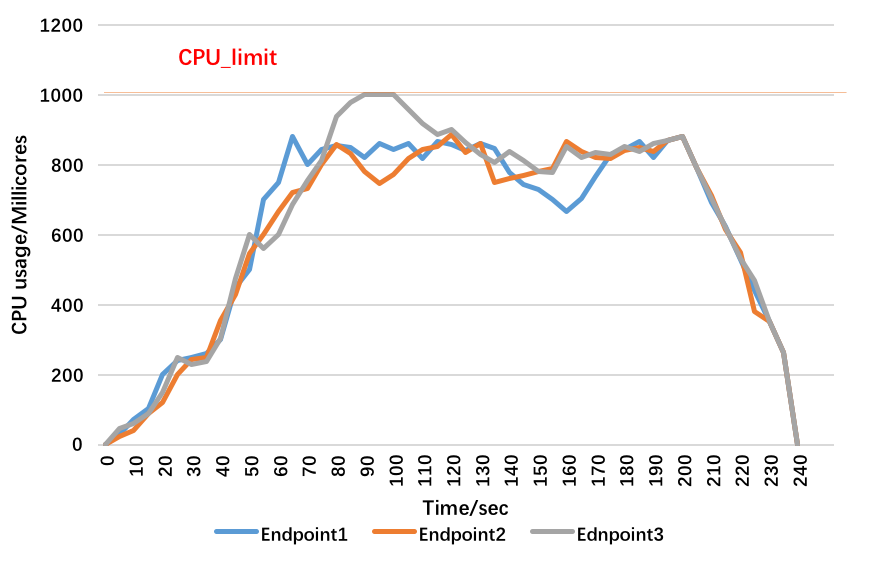
\includegraphics[width=0.45\textwidth]{images/data1.png}\\
  \caption{original controller under initialization pattern}
  \label{fig:original_initialization}
\end{figure}

\begin{figure}[!htb]
  \centering
  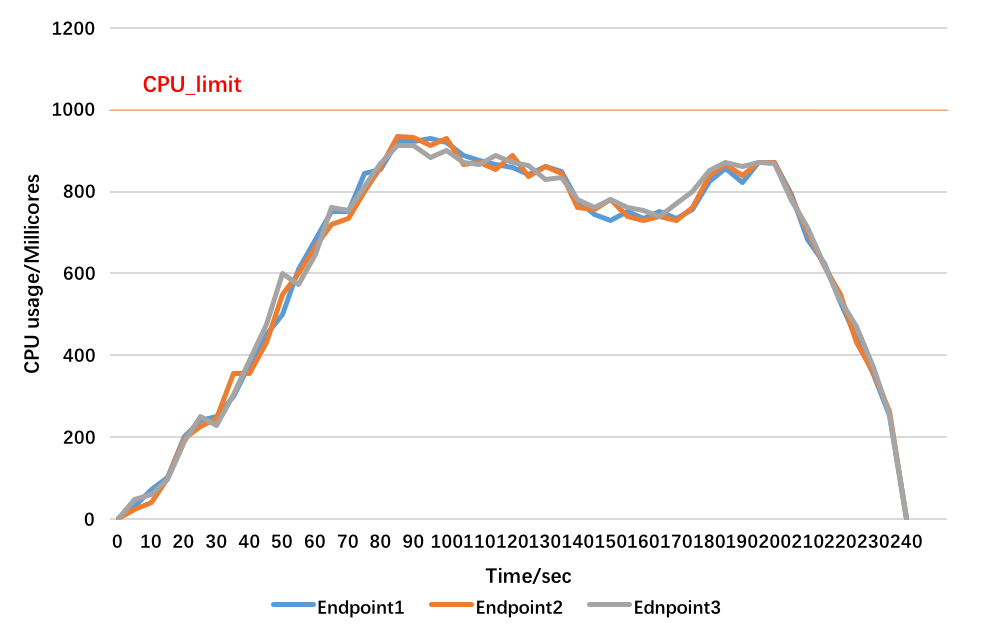
\includegraphics[width=0.45\textwidth]{images/data2.png}\\
  \caption{modified controller under initialization pattern}
  \label{fig:modified_initialization}
\end{figure}

Initialization pattern stands for the initial state when test applications are just deployed: we first deploy three replicas of test application, that is endpoint1 in node3, endpoint2 in node4 and endpoint3 in node5
to prevent that they are impacted by each other. After the deployment, we generate requests of all kinds at a fixed speed by tsung server to access test applications through ingress controller.
For convenience, we use the cpu statistics to present performance. Figure~\ref{fig:original_initialization} presents the performance of original ingress controller under initialization pattern and
figure~{\ref{fig:modified_initialization}} shows the performance of modified ingress controller. Result shows that for the original controller, load of endpoints become unstable and endpoint3 once becomes overhead(its cpu usage excceed its cpu limit) during 80s-100s, causing several
requests return 503 to tsung server, it confirms that the default round-robin algorithm only performs well when resource consumption of requests are almost the same, which is unpracticial. Figure~{\ref{fig:modified_initialization}} shows that
with the effort of modified ingress controller, there is no more overhead endpoint, load of endpoints are more even instead. More and more, table~{\ref{table:request_summary1}} points out that original ingress controller finishes 8892 reqeust, with 1108 503 requests, the
modified ingress controller finishes 10000 requests with no 503 request, and the total number of requests is 10000.
\hspace{0pt}
\begin{table}[htbp]
 \begin{center}
  \begin{tabular}{c|c|c|c}
   \hline
              & Finished    & 503   & Total  \\  \hline
   Original           & 10000   & 0   & 10000 \\ \hline
   Modified      & 8892     & 1102    & 10000    \\ \hline
  \end{tabular}
 \end{center}
 \caption{Request summary of initialization pattern}
 \label{table:request_summary1}
\end{table}
Throughout all cases, the FPS of full reconstruction policy is between 100 and 200.
\name{} shows a worse performance than \gvirt{} in cases without the Massive Update Issue, while achieving a better performance when the issue occurs.
As we discussed in section~\ref{subsec:recon_policy}, all 512 pages are applied with the relaxed mechanism, so full reconstruction brings more overhead
on reconstructing non-accessed pages, which is the reason for cases with little page update showing poor performance.

\begin{figure}[!htb]
  \centering
  \includegraphics[width=0.45\textwidth]{figure/static.eps}\\
  \caption{\name{} with static reconstruction policy}
  \label{fig:static}
\end{figure}

We selectively switch 50, 100, 200, and 300 pages into the relaxed mechanism to evaluate the static partial reconstruction policy.
As shown in Figure~\ref{fig:static}, for cases without the issue static partial reconstruction policy achieves a worse performance than \gvirt{}.
The more pages that are switched into the relaxed mechanism, the worse the performance static partial reconstruction becomes.
For pages with few page table updates, reconstruction is meaningless. For cases with the Massive Update Issue, the static partial reconstruction
policy works and achieves a superior performance than \gvirt{}. Policy with 200 pages setting achieves the best performance for cases with the
Massive Update Issue, because policies with less pages cannot cover all the frequently accessed pages,
and policies with more pages include some useless pages.


\begin{figure}[htbp]
  \centering
  \includegraphics[width=0.45\textwidth]{figure/partial.eps}\\
  \caption{\name{} with dynamic partial reconstruction and dynamic segmented partial reconstruction}
  \label{fig:partial}
\end{figure}

Figure~\ref{fig:partial} confirms that the dynamic segmented partial reconstruction achieves better performance than dynamic partial reconstruction
comprehensively. \name{} performs better than \gvirt{} in issued cases, and has similar performance in normal cases.
The dynamic partial reconstruction switches the PTE pages into the relaxed mechanism progressively. However, some pages switched into the relaxed mechanism
may never be accessed again, and reconstructing these pages will produce extra overhead. Dynamic segmented partial reconstruction resets the relaxed pages,
after setting them to the guest pages. So for each cycle, dynamic segmented policy only reconstructs pages that need to be reconstructed.
Overall, dynamic segmented partial reconstruction is the most efficient policy, which is finally adopted by \name{}.

\subsection{2D and 3D performance}
In this section, we evaluate the 2D and 3D performance of \name{} under Linux and Windows. The results show
that \name{} has comparable performance with \gvirt{}'s 2D and 3D performance.
Moreover, \name{} achieves slightly superior performance than \gvirt{} in some cases.

\begin{figure}[htbp]
  \centering
  \includegraphics[width=0.45\textwidth]{figure/linux.eps}\\
  \caption{Performance running Linux 2D/3D workloads}
  \label{fig:linux}
\end{figure}

\begin{figure}[htbp]
  \centering
  \includegraphics[width=0.45\textwidth]{figure/windows.eps}\\
  \caption{Performance running Windows 2D/3D workloads}
  \label{fig:windows}
\end{figure}
\hspace{0pt}

Figure~{\ref{fig:linux}} demonstrates that \name{} achieves up to 94.63\% of native performance in 2D workloads and 88.81\% in 3D workloads on Linux.
Figure~{\ref{fig:windows}} demonstrates that \name{} achieves up to 88.81\% on Windows.

With the exception of the firefox-scrolling, urbanterror, warsow, SM2.0 and Pass2D, \name{} outperforms \gvirt{}. However,
the performance discrepancy between \name{} and \gvirt{} are acceptable.

\section{Related Work}
\label{sec:related_work}

\subsection{\gpu{} Benchmarks}

\hspace{0pt}
Since \gpu{}s are used for acceleration of general purpose computing, some benchmarks have been implemented for evaluating their performance. Rodinia~{\cite{che2009rodinia}} is a benchmark suite for heterogeneous computing. It aids architects in the study of emerging platforms such as \gpu{}s. Rodinia includes applications and kernels that target multi-core CPU and GPU platforms. And Parboil~{\cite{stratton2012parboil}} is a set of throughput computing applications useful for studying the performance of throughput computing architecture and compilers.† It collects benchmarks from throughput computing application researchers in many different scientific and commercial fields including image processing, bio-molecular simulation, fluid dynamics, and astronomy.

Unfortunately, the benchmarks above are not available for Intel's GPU now. Meanwhile, GPU's media performance has become a big concern for service providers. However, there is no benchmark specifically for this kind of workload. So, this paper proposes GMedia, a media transcoding benchmark based on Intel's MSDK.

\subsection{\gpu{} Virtualization}

Though virtualization has been studied extensively in recent years, \gpu{} virtualization is still a nascent area of research. Typically, there are four ways to use \gpu{} in a \vm{}: I/O pass-through, device emulation, API remoting, and mediated pass-through.

A naive way to use \gpu{} in virtualized environment would be to directly pass through the device to a specific \vm{}~{\cite{hiremane2007intel, dong2009towards}}. However, the \gpu{} resources are dedicated and cannot be multiplexed.

Device emulation, similar to binary translation in CPU virtualization, is impractical. \gpu{}s, unlike CPUs, whose specifications are not well documented, vary between vendors~{\cite{dowty2009gpu}}. Emulating \gpu{}s from different vendors requires vast engineering work. Notably, following up the new \gpu{} hardware would make it a nightmare to maintain the codebase.

API remoting is widely used in commercial softwares such as VMWare and VirtualBox, and has been studied throughout many years. By using API remoting, graphic commands are forwarded from guest OS to host. VMGL~{\cite{lagar2007vmm}} and Oracle VirtualBox~{\cite{website:vbox}}, both based on Chromium~{\cite{humphreys2002chromium}}, replace the standard OpenGL library in Linux Guests with its own implementation to pass the OpenGL commands to VMM. Nonetheless, forwarding OpenGL commands is not considered a general solution, since Microsoft Windows mainly uses their own DirectX API. Whether forwarding OpenGL or DirectX commands, it would be difficult to emulate the other API.
gVirtuS~{\cite{giunta2010gpgpu}}, VGRIS~{\cite{qi2014vgris}}, GViM~{\cite{gupta2009gvim}}, rCUDA~{\cite{duato2010rcuda}} and vCUDA~{\cite{shi2012vcuda}} use the same manner to forward CUDA and OpenCL commands, solving the problem of virtualizing GPGPU applications.

VMware's products consist of a virtual PCI device, SVGA \RNum{2} card~{\cite{dowty2009gpu}}, and the corresponding driver for different operating systems. The emulated device acts like a real video card which has registers, graphics memory and a FIFO command queue. All accesses to the virtual PCI device inside a VM is handled on the host side, by a user-level process, where the actual work is performed. Moreover, they have designed another graphic API called SVGA3D. The SVGA3D protocol is similar to Direct3D and shares a common abstraction. The purpose of SVGA3D is to eliminate the commands for a specific GPU. Meanwhile, a \gpu{} can also emulate the missing features by SVGA3D protocol, which provides a practical portability for their products.

Recently, two full \gpu{} virtualization solutions have been proposed, i.e., \gvirt{} of Intel~{\cite{tian2014full}} and GPUvm~{\cite{suzuki2014gpuvm}}, respectively. \gvirt{} is the first open source product level full \gpu{} virtualization solution in Intel platforms. \gvirt{} presents a v\gpu{} instance to each VM which allows the native graphics driver to be run in VM. The shadow page table is updated with a coarse-grained model, which could lead to a performance pitfall under some video memory intensive workloads, such as media transcoding.

GPUvm presents a \gpu{} virtualization solution on a NVIDIA card. Both para- and full-virtualization were implemented. However, full-virtualization exhibits a considerable overhead for MMIO handling. The performance of optimized para-virtualization is two to three times slower than native. Since NVIDIA has individual graphics memory on the PCI card, while the Intel \gpu{} uses part of main memory as its graphics memory, the way of handling memory virtualization is different. GPUvm cannot handle page faults caused by NVIDIA \gpu{}s~{\cite{gottschlag2013logv}}. As a result, they must scan the entire page table when translation lookaside buffer (TLB) flushes. As \name{} allocates graphics memory within the main memory, VMM can write-protect the page tables to track the page table modifications. This fine-grained page table update mechanism mitigates the overhead incurred by the Massive Update Issue.

NVIDIA GRID~{\cite{website:nvidiagrid}} is a proprietary virtualization solution from NVIDIA for Kepler architecture. However, there are no technical details about their products available to the public.

\subsection{Memory Virtualization}

One important aspect in \gpu{} virtualization is memory virtualization, which has been thoroughly researched. The software method employs a shadow page table to reduce the overhead of translating a VM's virtual memory address. This approach could incur severe overhead under some circumstances. Agesen~\emph{et~al.}~{\cite{agesen2010evolution}} listed three situations where the shadow page table cannot handle well: the hidden page fault, address space switching, and the tracing page table entries. They also pointed out some optimization techniques, such as the trace mechanism and eager validating. Unfortunately, it is hard to trade off these mutually exclusive techniques. Therefore, AMD and Intel have added the hardware support for memory virtualization. All three overheads previously listed before can be eliminated, but it is not the silver bullet, a TLB miss punishment is higher in the hardware solution.
\hspace{0pt}
In the classical VMM implementations, VMM employs a trace technique to prevent its shadow PTEs from becoming inconsistent with guest PTEs, i.e. updating shadow page table strictly after the guest page table is modified. Typically, VM trace uses write-protection mechanism, which can be the source of overhead. This technique is similar to the current \gvirt{}'s strict page table shadowing mechanism, which frequently traps and emulates the page faults of the shadow page table, and it causes overhead. \name{} removes the write-protection from shadow page table to eliminate the overhead caused by excessive trap-and-emulation, taking advantage of the \gpu{} programming model~{\cite{adams2006comparison}}.

\section{Conclusion and Future Work}
\label{sec:conclusion}

\name{} is an optimized full \gpu{} virtualization solution, based on the Xen hypervisor, with the adaptive hybrid page table shadowing scheme, which improves performance for workloads with the Massive Update Issue when compared to \gvirt{}. To address this issue, this paper provides a hybrid page table shadowing scheme, i.e., strict and relaxed page table shadowing, to provide an optimized full GPU virtualization based on Xen hypervisor for Intel GPUs. \name{} combines these two page table shadowing mechanisms to reduce VM-exits to the hypervisor. Further, \name{} automatically switches page table between them by detecting \gpu{}'s current workloads, potentially showing significantly improvement to \gvirt{}'s performance for workloads with the Massive Update Issue. In order to decide what type of the page need to be reconstructed, four reconstruction policies are introduced. By running the same testcase through the four policies, the dynamic segmented partial reconstruction policy performs the best.

For future work, we will adapt \name{} to support KVM~{\cite{kivity2007kvm}} when \gvirt{} for KVM is ready. Additionally,  \name{} will be released in the open source community soon. We will focus on the areas of portability, scalability, and scheduling issues. With previous \gpu{} command scheduling methods, such as VGRIS and Pegasus~{\cite{deelman2005pegasus}}, we will investigate the low level access pattern of massive page table modification with the detailed analysis of the performance bottleneck of high level applications. We hope this optimized full \gpu{} virtualization solution gives insight into designing the support of efficient distributed systems for \gpu{} acceleration applications.

\section{Acknowledgements}
\label{sec:ack}
We thank  our shepherd Dan Tsafrir, Haibo Chen, and the anonymous reviewers for their insightful comments. This work was supported by National Science and Technology Major Project (No. 2013ZX03002004), National R\&D Infrastructure and Facility Development Program (No. 2013FY111900), NRF Singapore CREATE Program E2S2, and Shanghai
Key Laboratory of Scalable Computing and Systems. Prof. Haibing Guan is the corresponding author. 


\balance
{\footnotesize \bibliographystyle{acm}
\bibliography{HSCS}}


%\theendnotes

\end{document}
